%
% File: chap01.tex
% Author: Victor F. Brena-Medina
% Description: Introduction chapter where the biology goes.
%
\let\textcircled=\pgftextcircled
\chapter{Transient cavity dynamics and divergence from the Stokes–Einstein equation in organic aerosol}
\label{chap:water}


\section*{Contributions}

This chapter contains an adaption of ``Transient cavity dynamics and divergence from the Stokes–Einstein equation in organic aerosol'' by Young-Chul Song, Stephen Ingram, Robert E. Arbon, David O. Topping, David R. Glowacki, and Jonathan P. Reid. This was published in the journal Chemical Science, volume 11, pages 2999-3006. Copyright 2020 Royal Society of Chemistry. The article was published under a CC-BY license and so no special permission from the publishers was needed to reproduce the article here. 

Changes have been made including figures, section and reference numbers to suit a thesis structure and maintain formatting conventions with the rest of this thesis. Additional discussion of the results and conclusions have also been added. Some of the supplementary information from the paper has  been included in the main text, the remaining supplementary information can be found in appendix \ref{app:wat}. 

Contributions to the work: Young-Chul Song performed the experimental work; David O. Topping performed the analysis of diffusion constants from the experimental results; Stephen Ingram performed the MD simulations, the determination of the diffusion constants from MD simulations, the exploration of the cavity dynamics and the packing efficiency. The author of this thesis contributed to sections \ref{sec:wat_mech}, \ref{sec:wat_intro} and \ref{sec:wat_conclusions} of this work. Specifically: 
\begin{enumerate}
    \item Suggested the splitting of the molecular dynamics trajectories into times-slices, although did not do the analysis of the sucrose cavities (figure \ref{fig:wat_f3} and \ref{fig:wat_s8}). 
    \item Performed all Markov state modelling (exemplified in figures \ref{fig:wat_f4} and \ref{fig:wat_s10})) and wrote the Markov state modelling section of the supplementary material of the published paper, which has been incorporated into this chapter. 
    \item Classified the time-slices as being in equilibrium and non-equilibrium, and calculated the water hopping barrier heights (figure \ref{fig:wat_s9}) for the equilibrium time-slices. 
    \item Added discussion of Markov state models to the introduction (section \ref{sec:wat_intro}) and of the Markov analysis to the conclusions (section \ref{sec:wat_conclusions}). 
\end{enumerate}
The work was supervised by David R. Glowacki and Jonathan P. Reid. 

% \section{Introduction}
% Much of the recent work \cite{schererVariationalSelectionFeatures2019,husicMarkovStateModels2018} in Markov modelling has been on the feature selection problem: creating variationally optimised basis sets which capture the slow dynamics of the system. However, Markov models (MMs) still provide a powerful means of analysing MD simulations even when an adequate basis set is simple to define and variational optimisation is not needed. This chapter describes an experiment and computational investigation of the phenomenology of water transport in systems where the typical solvent/solute size relationship is reversed: small water `solute' molecules moving through a matrix of large organic `solvent' molecules.  Section \ref{sec:wat_paper} adapts the published version of this work, including supplementary information on the MMs.  Section \ref{sec:wat_commentary} discusses this work in terms of the larger body of MM research draws conclusions. 


% \section{}\label{sec:wat_paper}
\section{Introduction}\label{sec:wat_intro}
Examining the relationship between the diffusion rates of small molecules and the viscosity of the surrounding molecular matrix is important for exploring problems as diverse as the molecular mechanisms of crystallization and the formation of amorphous phases in drying droplets \cite{Nascimento2010,Mikhailov2009a,Koop2011}, the controlled-release of active ingredients from structured micro-particles in pharmaceutical and consumer products \cite{hidy1984aerosols,Hancock1997,Lorenz2011,Haddrell2014}, and the mass concentration of secondary organic aerosol particles in a polluted urban environment \cite{Shiraiwa2012a,mai2015under,Maclean2017}. The simplest relationship, the Stokes–Einstein (S–E) equation, expresses the inverse correlation between the translational diffusion coefficient, $D$, of a large spherical solute molecule of radius $a$, moving within a solvent continuum with a dynamic viscosity, $\eta$ \cite{powerTransitionLiquidSolidlike2013,chenStokesEinsteinRelationSupercooled2006}:
\begin{equation}\label{eqn:diffusion}
D=\frac{k_{\mathrm{B}} T}{C \pi \eta a}
\end{equation}
where $C$ is a constant. However, in many important cases the ``solvent” (i.e. the dominant component by mole fraction) may be a large organic molecule and the ``solute” (i.e. the minor component) may be a small molecule, e.g. water \cite{powerTransitionLiquidSolidlike2013,Price2014,Molinero2005}. For example, in the drying of aqueous-organic solution droplets, the evaporation of water can lead to an involatile solute surpassing its solubility limit, thereby becoming the major component with a mole fraction that can approach $1$. The sudden removal of water can lead to a ``frozen'' organic-rich matrix with a sufficiently high viscosity such that nucleation and crystallization are delayed, unable to occur on an experimentally realisable timescale, with the solution composition crossing the threshold for a moisture-induced glass transition \cite{Bones2012}. Even then, the residual moisture content can impact product lifetime and particle morphology. Under these conditions, it is most appropriate to consider the diffusion of water within an organic matrix at infinite dilution of water; however, it is typical that a significant divergence from the S–E equation is observed in this limit \cite{powerTransitionLiquidSolidlike2013,Price2015,Chenyakin2017}. Modifications to the S–E equation have been suggested, including the use of a fractional exponent (i.e. $D \propto \eta^{-\alpha}$), that account for different relationships between the diffusion coefficient and viscosity \cite{Harris2009,price2016sucrose, Fernandez-Alonso2007}.

Independent measurements of diffusion coefficients and viscosities over the appropriately wide ranges needed to observe the failure of the S–E equation are challenging. Most measurements report the temperature-dependence of viscosities and diffusion coefficients for super-cooled liquids or solutions of fixed composition, and can approach close to the glass transition temperature \cite{chenStokesEinsteinRelationSupercooled2006,Shrestha2015,Chen2006a,Gonzalez2015}. By contrast, there are many fewer studies of the compositional dependence of the divergence from the S–E equation, for example with diminishing moisture content as the glass transition relative humidity (RH) is approached \cite{powerTransitionLiquidSolidlike2013,Price2014,Price2015,Chenyakin2017,price2016sucrose,Bastelberger2017a}. Moisture acts as a plasticizer in atmospheric aerosol particles, regulates the viscosity and, thus, shelf-life of amorphous particles used in formulations, and could play a critical influence in governing crystal formation in drying droplets and films as opposed to the formation of an amorphous solid. Examining the compositionally dependent divergence of an organic solute–water mixture from S–E behaviour not only requires accurate measurements of diffusion coefficients and viscosities over as much as \num{15} orders of magnitude but requires accurate measurements of composition, recognising that both viscosity and diffusion coefficients are highly dependent on the identity for the functional groups forming the organic solute \cite{rothfuss2017influence}. To access the full viscosity range, moisture must be removed from metastable supersaturated solution droplets without crystallization. 

Reported here is a systematic experimental and computational study of the failure of the S–E equation for a range of aqueous-saccharide solutions, varying the molecular size of the organic molecule forming the viscous matrix relative to water and exploring the detailed mechanism of water transport in the limit of a pure saccharide particle. The experimental measurements are complemented with \SI{9}{\micro\second} of molecular dynamics (MD) simulations at atomistic resolution for a single type of saccharide matrix.  In order to understand the microscopic dynamics of the water transport a Markov model (MM) approach was used. Much of the recent work \cite{schererVariationalSelectionFeatures2019,husicMarkovStateModels2018} in Markov modelling has been on the feature selection problem: creating variationally optimised basis sets which capture the slow dynamics of the system. However, this work uses the Cartesian coordinates of the water molecule, with no variational optimisation, as a method for both i) partitioning and classifying the dynamics as being in either local equilibrium or non-equilibrium and, ii) determining the typical free energy barriers faced by water as it moves through the saccharide matrix. This chapter is structured as follows. In section \ref{sec:wat_d_coefs} the experimental measurements of diffusion coefficients are described and discussed; section \ref{sec:wat_d_eta} makes the link  between the diffusion and viscosity; section \ref{sec:wat_mech} describes the elucidation of the microscopic mechanism from molecular dynamics simulations and MMs; section \ref{sec:wat_conclusions} concludes and discusses limitations of the Markov modelling. 

\section{Measurements of diffusion coefficients of water in aqueous-saccharide aerosol particles}\label{sec:wat_d_coefs}

Not only are saccharides used widely as excipients for drug delivery \cite{Zhao2009,Sinha2001,Sastry2000} and excipient particles are often prepared by spray drying \cite{Andya1999,Vehring2008,Mosen2004}, they find widespread application in the food industry and are commonly used as laboratory surrogates for high oxidized viscous secondary organic atmospheric aerosol \cite{Koop2011,Bones2012,Liu2006,Zobrist2008,Reid2018,Song2016a}. Using aerosol particles levitated in optical tweezers, measurements were  carried out  which avoid the process of heterogeneous nucleation that occurs in the presence of a substrate, allowing access to particle viscosities spanning dilute aqueous solutions (\SI{10}{\milli\pascal\second}) to an amorphous solid (\SI{10}{\tera\pascal\second}). The moisture content is readily altered by varying the relative humidity of the gas phase. Specifically, considered here are five binary aqueous-saccharide solution aerosols: glucose (a mono-saccharide); sucrose, trehalose and maltose (all di-saccharides); and raffinose (a tri-saccharide). Also considered are aqueous aerosol droplets containing levoglucosan, a representative oxygenated compound of biomass burning aerosol particles in the atmosphere \cite{Decesari2006}.

\begin{figure}
    \centering
    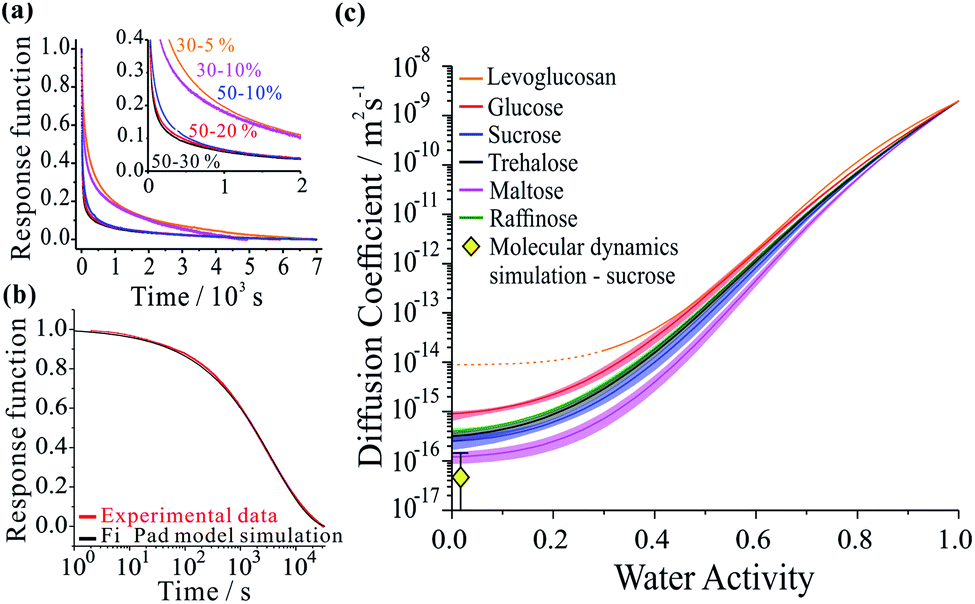
\includegraphics[width=0.8\textwidth]{chapters/water_hopping/figures/f1.png}
    \caption[Example experimental workflows]{\textsc{Example experimental workflows}. Examples of each step in the workflow required to extract the compositional dependencies the diffusion coefficients from a time-dependence in particle size. The panels show: (a) a collection of response functions for size changes of aqueous-raffinose particles following a step change in RH; (b) a single response function following a change in RH from \numrange{30}{5} RH for a sucrose particle and the best-fit produced by the Fickian diffusion model. (c) The estimated compositional dependencies of the diffusion of water in the six binary aqueous-organic aerosol systems studied. The estimate of the diffusion coefficient for water in sucrose from the MD simulations also presented (yellow diamond).}
    \label{fig:wat_f1}
\end{figure}

 Figure \ref{fig:wat_f1} panel (a) shows examples of the time-dependence in the size response functions for aqueous-raffinose particles following transitions in RH. The significant changes in the equilibration time reflect the significant changes in particle viscosity that are observed over this range in RH/moisture content: equilibration at RHs above the glass-transition RH occurs on timescales $\ll \SI{1}{\hour}$; at low RH, the release of moisture from an amorphous glass occurs over many hours and indeed is not complete over the experimental timescales. The time-constant, $\tau$, and ``stretch factor” $\beta$ of the multiexponential decay observed in both evaporation and condensation events show a path dependence, varying with both the initial and final RH, the initial particle size and the wait-time at intermediate RHs (see figure \ref{fig:wat_s4}). Tabulated values of both parameters observed in each of the new systems may be found in table \ref{tab:wat_s1}. To fit the compositional/water activity dependence of the diffusion coefficient of water for binary solution aerosol droplets requires measurements at many RH transitions \cite{Ingram2017,Rickards2015}.
Measurements were performed over \num{6} RH transitions for \num{96} droplets for the six binary aqueous-organic aerosol systems studied (glucose, sucrose, trehalose, maltose, raffinose and levoglucosan). Transitions in size were slowest for maltose droplets at the lowest RHs. Moreover, the characteristic timescale increases with increasing particle size for every binary organic system studied (see figure \ref{fig:wat_s3} and table \ref{tab:wat_s1}). Time-constants for all particle sizes in the range \SIrange{3}{6}{\micro\meter} show the same ordering: maltose $>$ raffinose $>$ trehalose $>$ sucrose $>$ glucose $\ge$ levoglucosan. In other words, the chain length of the organic fraction appears to be important to the internal mixing dynamics but is not the only controlling factor.

The compositional dependencies of the diffusion coefficients of water estimated for these binary aqueous-organic systems are summarized in panel (c). For reference, the moisture driven glass transition RH has been reported as \SI{53}{\percent} for raffinose \cite{Song2016a,Tong2011} and \SI{32}{\percent} for maltose \cite{Song2016a}; the majority of evaporation measurements for these two systems have been made with ultra-viscous and even glassy particles. A value of \SI{23}{\percent} RH has been reported for sucrose \cite{Song2016a,Tong2011} while glucose and levoglucosan are not expected to become glassy at any moisture content at this temperature \cite{Zobrist2008}; indeed, levoglucosan crystalizes at an RH of \SI{30}{\percent} and diffusion coefficients cannot be measured below this. The trend in $D_{w}$ is not monotonic with molecular weight: levoglucosan (\SI{162.1}{\gram\per\mol}) $>$ glucose (\SI{180.2}{\gram\per\mol}) $>$ raffinose (\SI{504.4}{\gram\per\mole}) $>$ trehalose (\SI{342.3}{\gram\per\mole}) $>$ sucrose (\SI{342.3}{\gram\per\mol}) > maltose (\SI{342.3}{\gram\per\mole}) at the same water activity. Water in the monosaccharide shows the fastest diffusivity, and diffusion in the trisaccharide is faster than in the disaccharides when a fixed RH/water activity is considered. Indeed, this trend in the diffusion coefficient of water in the limit of a pure dry organic matrix is consistent with a previous assessment of the diffusion coefficients at the glass transition temperature for a subset of the compounds studied here \cite{lienhard2015viscous}.

\section{The relationship between diffusion and viscosity in mono-, di- and tri-saccharide particles}\label{sec:wat_d_eta}

The diffusion coefficient measurements presented in figure \ref{fig:wat_f1} and our measurements of solution droplet viscosities \cite{Song2016a} allow us to examine their correlation over wide ranges spanning more than \num{12} orders of magnitude in viscosity and \num{7} orders of magnitude in diffusion coefficient. The correlations for these systems are compared with predictions from the S–E equation in figure \ref{fig:wat_f2}, assuming a molecular diameter for water of \SI{0.2}{\nano\meter}. Typical error estimates in diffusion coefficient and viscosity are indicated by the representative error bars for each system. The diffusion coefficients for water in all organic-aqueous solutions increasingly deviate from the S–E equation with decreasing water activity and increasing viscosity. Even at the threshold of semi-solid behaviour (\SI{104}{\pascal\second}), the diffusion coefficient of water in aqueous-raffinose aerosol droplets is $\sim \num{5}$ orders of magnitude larger than estimated by S–E. This is a consequence of the inapplicability of the S–E assumptions to estimations of the diffusion coefficient of a small molecule moving within a matrix of large molecules, i.e. the translation of water is not characterized by simple Brownian motion \cite{Chen2006a,Liu2015}.

\begin{figure}
    \centering
    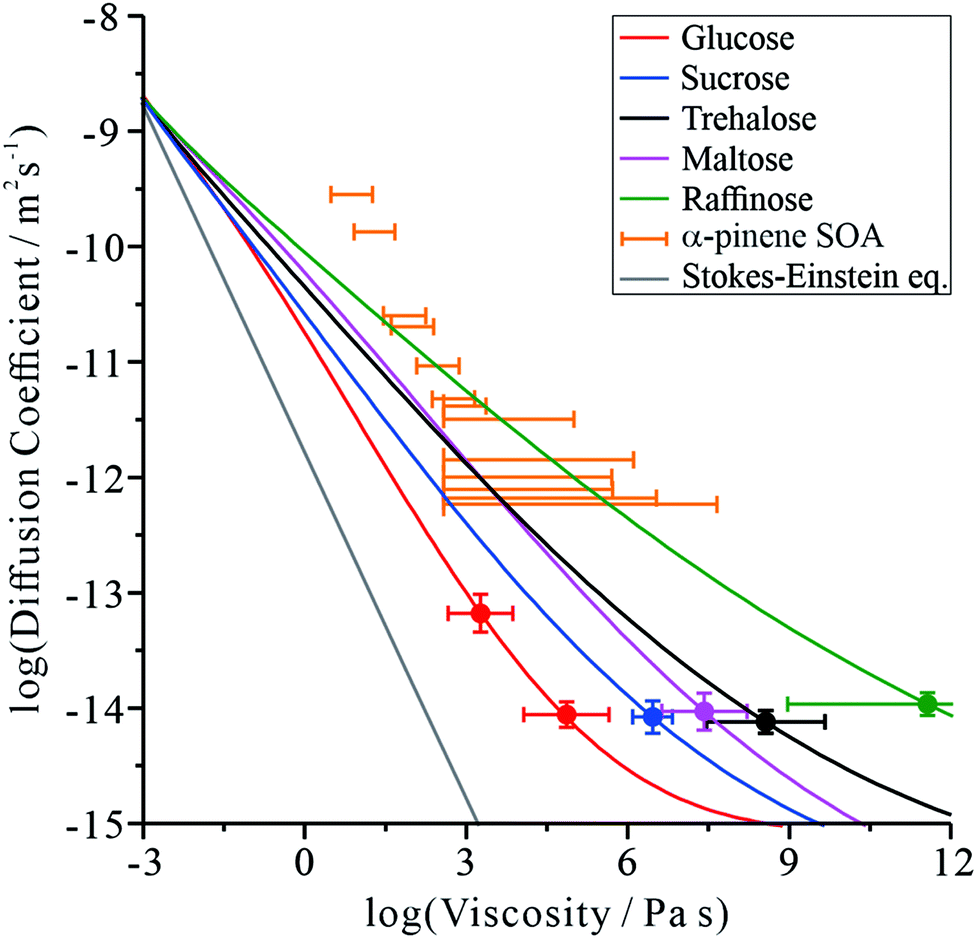
\includegraphics[width=0.8\textwidth]{chapters/water_hopping/figures/f2.png}
    \caption[Correlation of the diffusion coefficient of water with the viscosity of the aqueous-organic matrix]{\textsc{Correlation of the diffusion coefficient of water with the viscosity of the aqueous-organic matrix}.  A prediction from the S–E equation is shown by the grey line. The relationship between the diffusion constant and viscosity of $\alpha$-pinene SOA (orange markers) has been inferred by us from the literature, and has previously been discussed.\cite{Price2015,Chen2013} The colour scale is the same as in figure \ref{fig:wat_f1}.} 
    \label{fig:wat_f2}
\end{figure}

Comparing the relative divergence of water diffusion coefficients from S–E predictions for the mono-, di- and tri-saccharides, the discrepancy increases systematically across this series. Water transport is fastest in solutions with the tri-saccharide raffinose and slowest in solutions with the mono-saccharide glucose at a certain solution viscosity; the di-saccharides (sucrose, trehalose and maltose) fall in the intermediate range. These results suggest that the disparity in size between water and the organic molecule forming the matrix is key to determining the diffusion rate of water. It also explains why the particle size relaxation times and limiting $D$ values (in dry air) did not directly scale with molecular weight: the particles exhibit different viscosities at the same water activity. Therefore, an independent viscosity axis, in this case produced using the aerosol particle coalescence technique, is crucial to separating the two effects.

It can be postulated that when forming a matrix from raffinose, a much larger molecule than water, the packing density of raffinose leaves sufficient free volume for water to move more readily through the network of organic molecules. When the organic molecule is closer in size to water, as in the case of the mono-saccharide glucose, the tighter relative packing of glucose leads to a fewer adequately sized cavities. In this sense, the mechanism of impaired water transport more closely resembles percolation rather than diffusion \cite{Shante1971,Shiraiwa2011}, a process that is sensitive to the free volume of the medium \cite{White2016}.

Figure \ref{fig:wat_f2} is instructive when considering the diffusion of water through the complex organic matrices found in atmospheric secondary organic aerosol (SOA), one particular motivation for the current study. For example, water transport in $\alpha$-pinene SOA (orange bars) is more rapid than would be expected based on measurements of viscosity and estimates from the S–E equation \cite{powerTransitionLiquidSolidlike2013,Molinero2005,Price2015}, most closely resembling the di- and tri-saccharides. However, it should be recognised that the properties of SOA constituent molecules are considerably different. The average molecular weight of organic components identified in $\alpha$-pinene SOA is \SIrange{150}{200}{\gram\per\mole} \cite{Chen2013}, albeit with a lower degree of oxygenation: typically the O:C ratio has been reported as \numrange{0.45}{0.55} \cite{zhang2015formation}. The O:C ratios for trehalose and raffinose are \num{0.92} and \num{0.89}, respectively. The faster diffusion of water in SOA than expected from the S–E equation may be attributed to the heterogeneity in composition at the molecular scale, leading to a porous network of channels through which water transport is more facile than expected.

\section{The microscopic mechanism from molecular dynamics simulations}\label{sec:wat_mech}

To better understand the microscopic mechanism of water transport, atomistic molecular dynamics (MD) simulations of water in sucrose (with ‘concentrations’ of one water molecule per \num{35} sucrose molecules) were carried out which were designed to mimic experimental water activities close to zero. See appendix \ref{app:wat} for further information on the MD simulations. The initial placement of the organic molecules is intended to replicate the amorphous packing structure that is expected to occur near the surface of a glassy sucrose droplet \cite{Mikhailov2009a}. These MD simulations were analysed to provide an independent estimate for the value of the intercept $D_{\mathrm{w,org}}$. Figure \ref{fig:wat_f1} panel (c) shows the MD-derived value of \SI{4.64d-17}{\meter\squared\per\second} is in good agreement with the experimental measurements, and indicates that our computational approach captures the physics of water diffusion in sucrose at low activities.

\begin{figure}
    \centering
    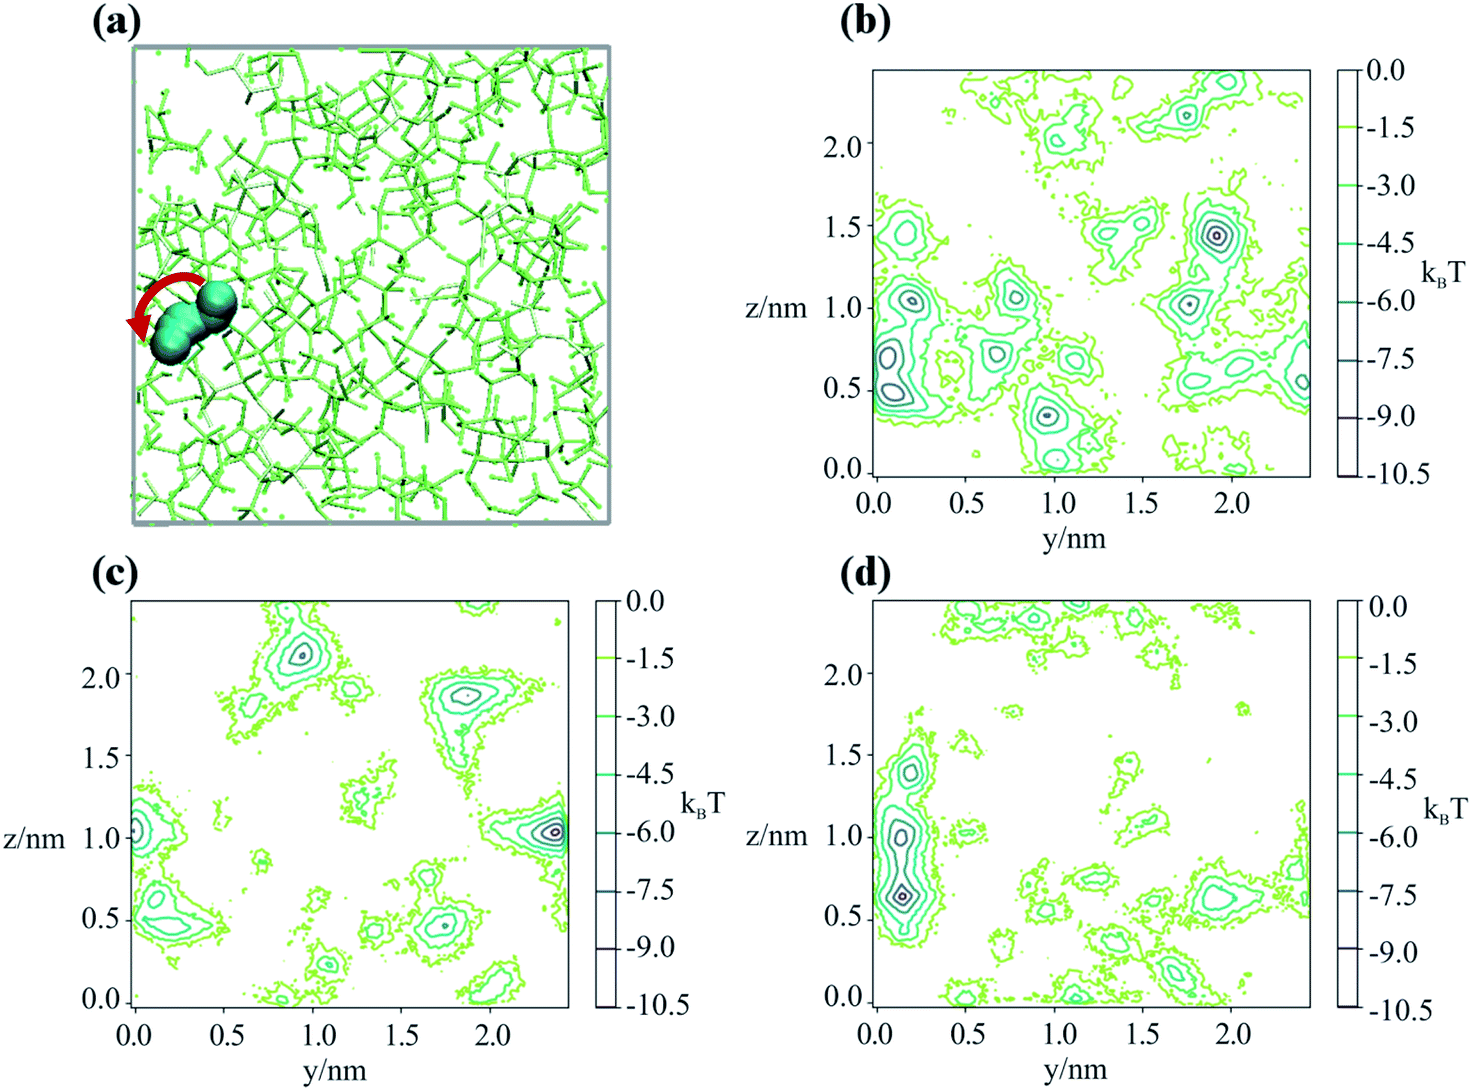
\includegraphics[width=0.8\textwidth]{chapters/water_hopping/figures/f3.png}
    \caption[Sucrose matrix cavities]{\textsc{Sucrose matrix cavities}. (a) Snapshots in the yz plane of the trajectory of a water molecule ‘jumping’ between interstices in an amorphous sucrose lattice. The red arrow indicated the direction of the observed hop. The periodic box is shown in grey. Sequential calculated potentials of mean force that the water experiences are shown in panels (b) to (d), separated in time by \SI{1}{\nano\second}.}
    \label{fig:wat_f3}
\end{figure}

Inspection of our MD results reveals that the mechanism of water diffusion through the sucrose matrix proceeds by a hopping between cavities (figure \ref{fig:wat_f3}). In general, a `cavity’ is defined as a sucrose interstitial domain where water has a significant lifetime based on Markov analysis. Our analysis has enabled us to identify both reversible and irreversible examples of intercavity dynamics. Figure \ref{fig:wat_f4} and much of the analysis described in this article focuses on clusters of `cavities’ between which water molecules make reversible kinetic hops, because this local equilibrium is amenable to analysis using standard tools in statistical mechanics.

\begin{figure}
    \centering
    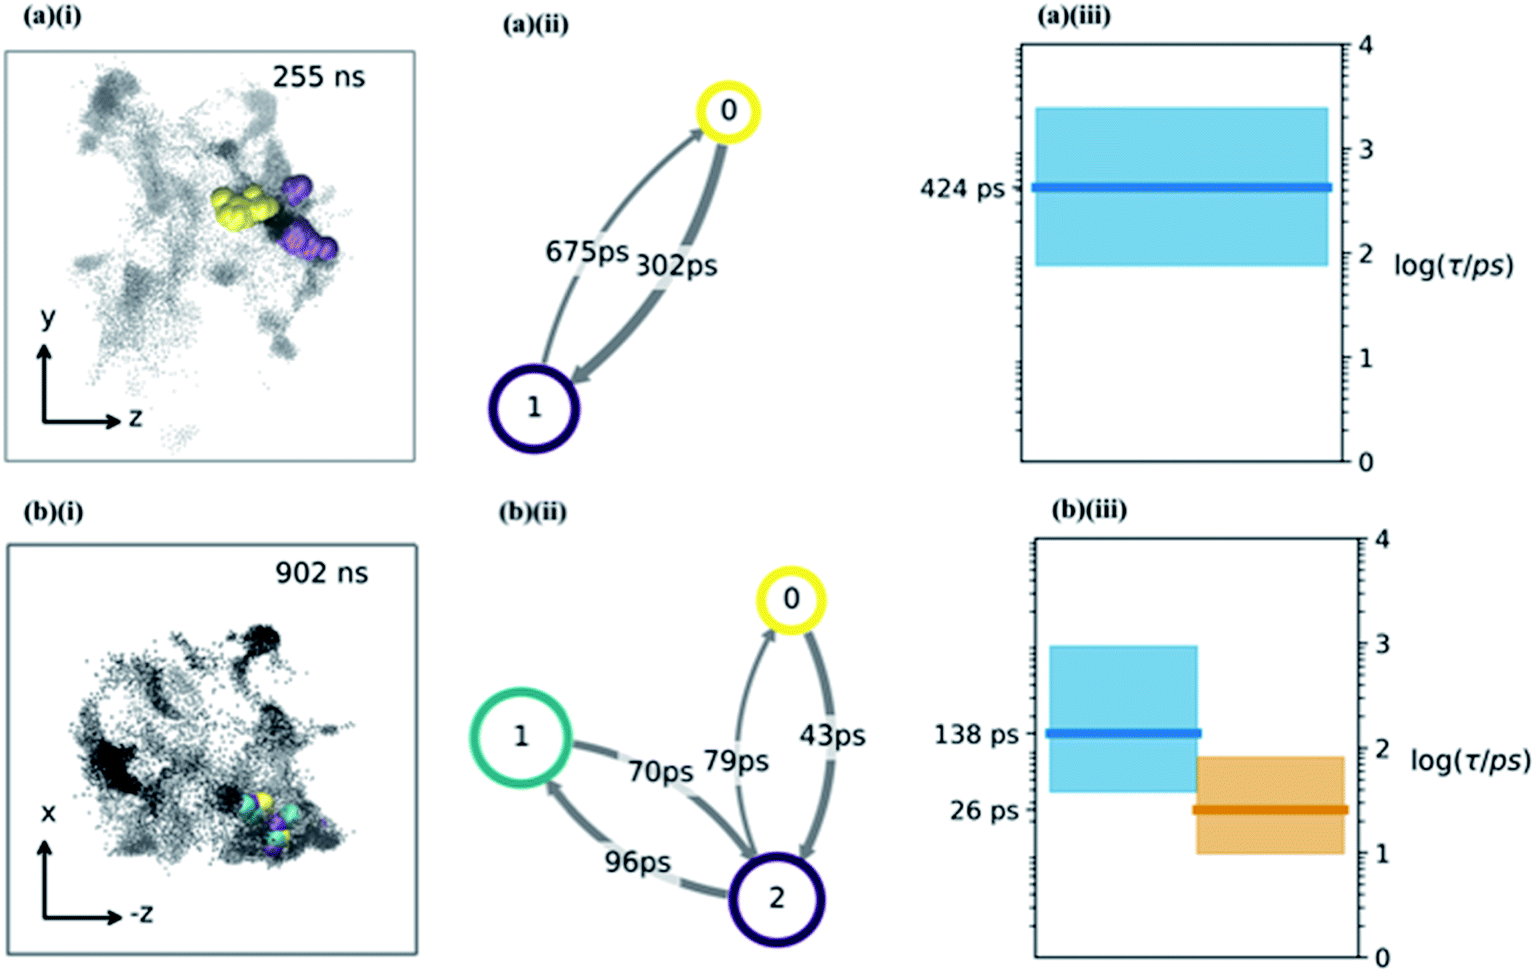
\includegraphics[width=0.8\textwidth]{chapters/water_hopping/figures/f4.png}
    \caption[The water hopping mechanism]{\textsc{The water hopping mechanism}. (a and b) The water hopping mechanism showing 2 and 3 metastable states (panels (a) \& (b) respectively) arising from one of the nine trajectories. Subplots (i) show zy, (-z)x projections of water molecule's position throughout the trajectory with different colours indicating different metastable states. Subplots (ii) shows a hidden Markov state model representation of the hopping behaviour. Each circle represents a metastable state, with the size related to its stability, the arrows show the hopping timescale in picoseconds from one state to another (same colour scheme as (i) subplots). Subplots (iii) show Bayesian estimates of the relaxation timescales associated with hopping between the states (thick line is mean, coloured region is a \SI{95}{\percent} credibility interval).}
    \label{fig:wat_f4}
\end{figure}

Our analysis shows that water remains in a cavity (or cluster of cavities) until either (1) it achieves sufficient kinetic energy to escape the local environment, or (2) the slower dynamics of the sucrose matrix opens a pathway that allows access to a new cavity. This appears similar to the `micropore diffusion’ mechanism, which has been proposed to describe the uptake and transport of small molecules through porous zeolite structures \cite{Krishna1997}.

In order to determine the time-dependent dynamics of the cavities, a \SI{3}{\nano\second} timeslice of a \SI{1}{\nano\second} trajectory was identified, where a water molecule jumping between two distinct cavities was observed, as illustrated in figure \ref{fig:wat_f3} panel (a). Over the course of the \SI{3}{\nano\second} timeslices,  three different equilibrium configurations were extracted, and a \SI{50}{\nano\second} MD simulation beginning from each of these points was run, freezing the sucrose but not the water. The purpose of these simulations was to use the water molecular as a ``probe'' of the cavity structure and dynamics, in order to understand cavity persistence on the timescale of a typical water hop. The potential of mean force within each cavity (PMF), without the entropic degrees of freedom of the organic matrix included, was determined by Boltzmann weighting the resultant probability distribution, $P$: 

\begin{equation}\label{eqn:pmf}
\mathrm{PMF}=-k_{\mathrm{B}} T \ln (P)
\end{equation}

\begin{figure}
    \centering
    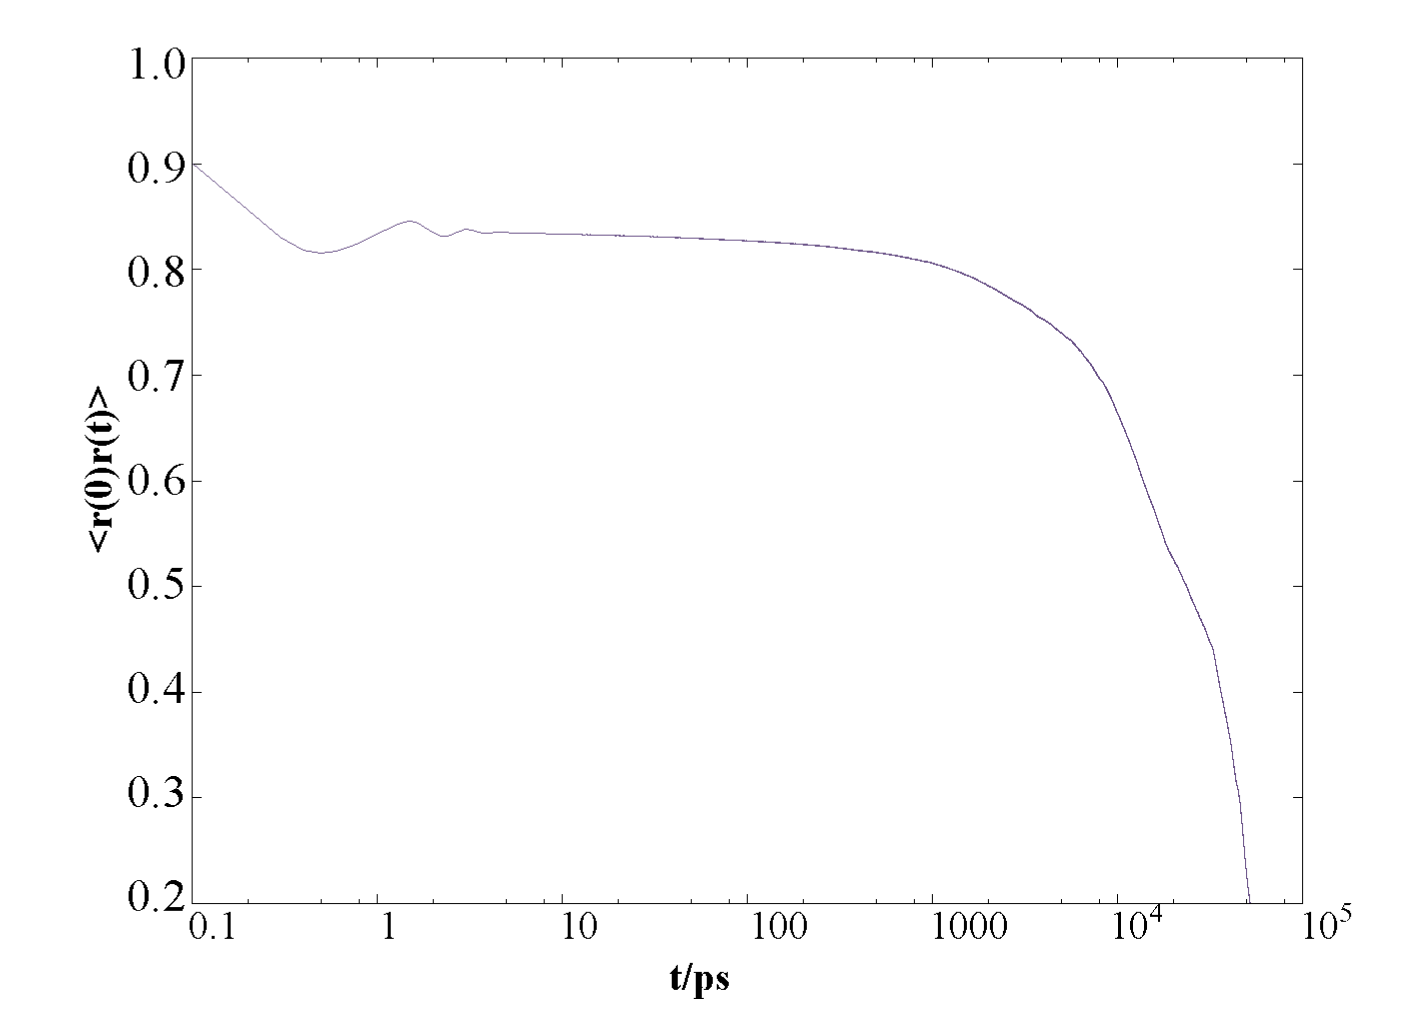
\includegraphics[width=0.8\textwidth]{chapters/water_hopping/figures/Fig_S8.png}
    \caption[Position-position autocorrelation function of a single sucrose molecule within the simulation]{\textsc{Position-position autocorrelation function of a single sucrose molecule within the simulation}. The plot shows very little motion in the region \SIrange{0.1}{1000}{\pico\second}.This plot suggests that it is reasonable cluster the data (to determine cavities, as in figure \ref{fig:wat_f4}) in increments of \SI{1}{\nano\second}. It is also reasonable to initialise frozen sucrose simulations after intervals of \SI{1}{\nano\second} (figure \ref{fig:wat_f3}, panels (b) - (d))}
    \label{fig:wat_s8}
\end{figure}

Figure \ref{fig:wat_f3} panels (b) to (d) shows that there is a small but noticeable change in the cavity PMF landscape (the region around $y = 0.1$, $z = $\numrange[range-phrase=--]{0.5}{1}) as the sucrose reorients over \SI{3}{\nano\second}. This observation is consistent with analysis showing that the position–position autocorrelation function of a single sucrose molecule decorrelates after approximately \SI{1}{\nano\second}, as presented in figure \ref{fig:wat_s8}.  Having determined an approximate upper limit on the sucrose re-organisation timescale,  each trajectory was split up into \SI{1}{\nano\second} slices and  the kinetic parameters for water-hopping between cavities were determined using a Bayesian Hidden Markov (HM) modelling approach. 

The sucrose reorganisation time of \SI{1}{\nano\second} defines a time scale over which the molecular environment, which defines the free energy surface over which the water moves, remains stationary.  Over this time scale the rates of water diffusion can be assumed to be independent of time, which admits a Markov analysis (where the transition rates do not vary with time).  Within these stationary time-slices, the water molecule was typically observed to remain trapped within a small region made up of one or more cavities as shown in figure \ref{fig:wat_f3}.  The dynamics of the water molecule can be classified as either reversible or irreversible with respect to these small regions.  If the dynamics were reversible then the absolute probability of observing hops from one part, $A$, of the region to another part $B$, of the region (between two cavities within the region, or within a single cavity) is the same $A\rightarrow B$ and $B\rightarrow A$. In other words, detailed balance is observed when concentrating on only one time-slice.  If this criteria is not fulfilled, the dynamics were said to be irreversible. 

The goal of the Markov modelling was to identify regions of the MD simulations in local equilibrium,to identify cavities,and calculate their associated hopping and relaxation timescales. Eight MD simulations were partitioned into \SI{1}{\nano\second} time-slices and the position of the water center of mass was clustered into $100$ discrete states using the k-means \cite{lloydLeastSquaresQuantization1982} clustering algorithm. A Markov lag time of $\tau_{M} = \SI{10}{\pico\second}$ was used based on the implied timescales of $10$ randomly selected time-slices from trajectory \num{3}.  The k-means clustering and all subsequent calculations were performed using the open source software, PyEMMA (version 2.5) \cite{schererPyEMMASoftwarePackage2015a}. 

\begin{figure}[p]
    \centering
    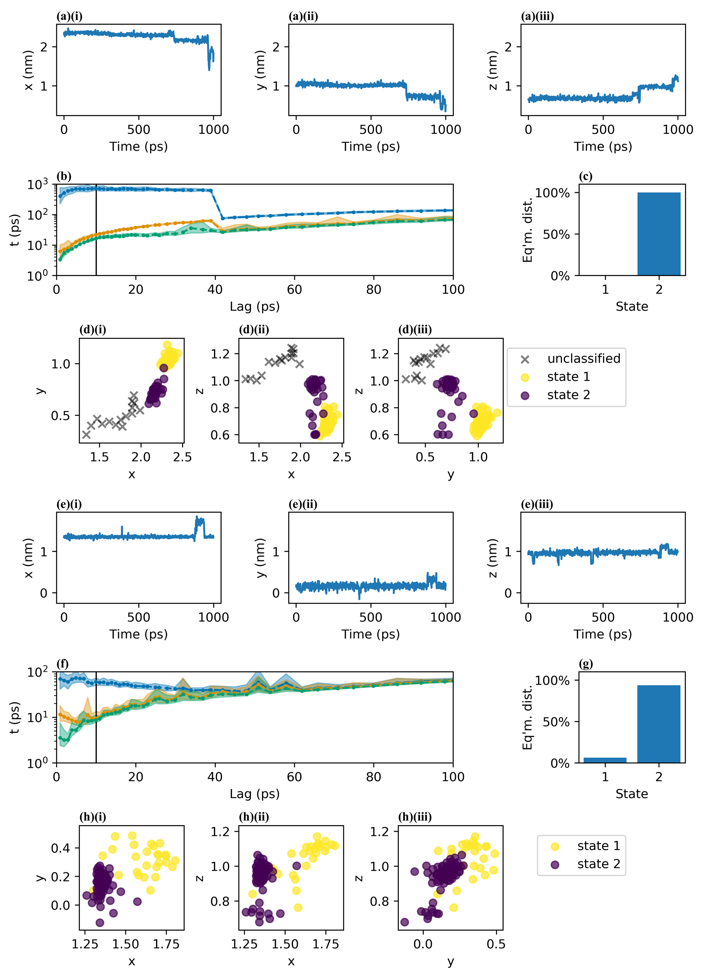
\includegraphics[width=0.8\textwidth]{chapters/water_hopping/figures/Fig_S11.png}
    \caption[Classification of two time-slices from trajectory 3]{\textsc{Classification of two time-slices from trajectory 3}: \SIrange{0}{1}{\nano\second} (panels (a) - (d), non-equilibrium time-slice) and \SIrange{22}{23}{\nano\second} (panels (e) - (h), local equilibrium time-slice). Panel (a) and (e) show the $x$, $y$, and $z$ coordinates of the center of mass of the water molecule. Panel (b) and (f) show the sensitivity analysis to determine the lag time $\tau_{M}$: the implied timescales, ($t$ vertical axis) vs the MSM lag, ($\tau_{M}$ horizontal axis). The black vertical line is placed at \SI{10}{\pico\second} is the minimum time at which the implied timescales show convergence. Panels (c) and (g) show the stationary distribution. In panel (c) state $1$ has negligible probability classifying this time-slice as not being in equilibrium. Panels (d) and (h) show the attempted assignment of the discrete trajectory into metastable states. The non-equilibrium time-slice in panel (d) shows the large portion of unclassified states.}
    \label{fig:wat_s10}
\end{figure}

The discrete trajectories were screened to see whether they were in local equilibrium with the following procedure:
\begin{enumerate}
    \item A Markov state model (MSM) with a lag time ($\tau_{M}$) of \SI{10}{\pico\second} was constructed for each time-slice. The lag time was chosen so as to reveal details of potential metastability \cite{prinzMarkovModelsMolecular2011}. To determine the value of $\tau_{M}$  a sensitivity analysis was carried out, varying $\tau_{M}$ until convergence was observed  in the timescales. See figure \ref{fig:wat_s10} panel (b) \& (f).
    \item This MSM was coarse grained into a $k$-state Hidden Markov Model (HMM) if the largest gap in successive implied timescales of the MSM $\left(t_{k} / t_{k+1}\right)$ was greater than \num{1.5}. 
    \item If the HMM had:
    \begin{enumerate}
        \item an absorbing state (a \num{1} on the diagonal of the transition matrix);
        \item an metastable state, $i$, with stationary distribution $\left(\pi_{i}\right)$ probability approximately zero $\left(\pi_{i}< 10^{-8}\right)$
        \item negative eigenvalues; 
    \end{enumerate}
    it was classified as not being in local equilibrium.The conditions (a) – (c) are indicative of not being in equilibrium because of the enforcement of the detailed balance conditions when estimating the HMM transition matrix \cite{noeProjectedHiddenMarkov2013a}.
    \item The time-slices identified as being in local equilibrium were used to construct a Bayesian HMM in order to estimate errors of the hopping timescales. 
\end{enumerate}

Out of the \num{8000} time-slices analysed \num{947} (\SI{11.8}{\percent}) were positively identified as being in local equilibrium. Figure \ref{fig:wat_s10} demonstrates this classification algorithm for two time-slices of trajectory \num{3}. The first time-slice (\SIrange{0}{1}{\nano\second}, panels (a) to (d)) was classified as not being in local equilibrium, the second time-slice (\SIrange{22}{23}{\nano\second}, panels (e) - (h)) was classified as being in local equilibrium.

\begin{figure}
    \centering
    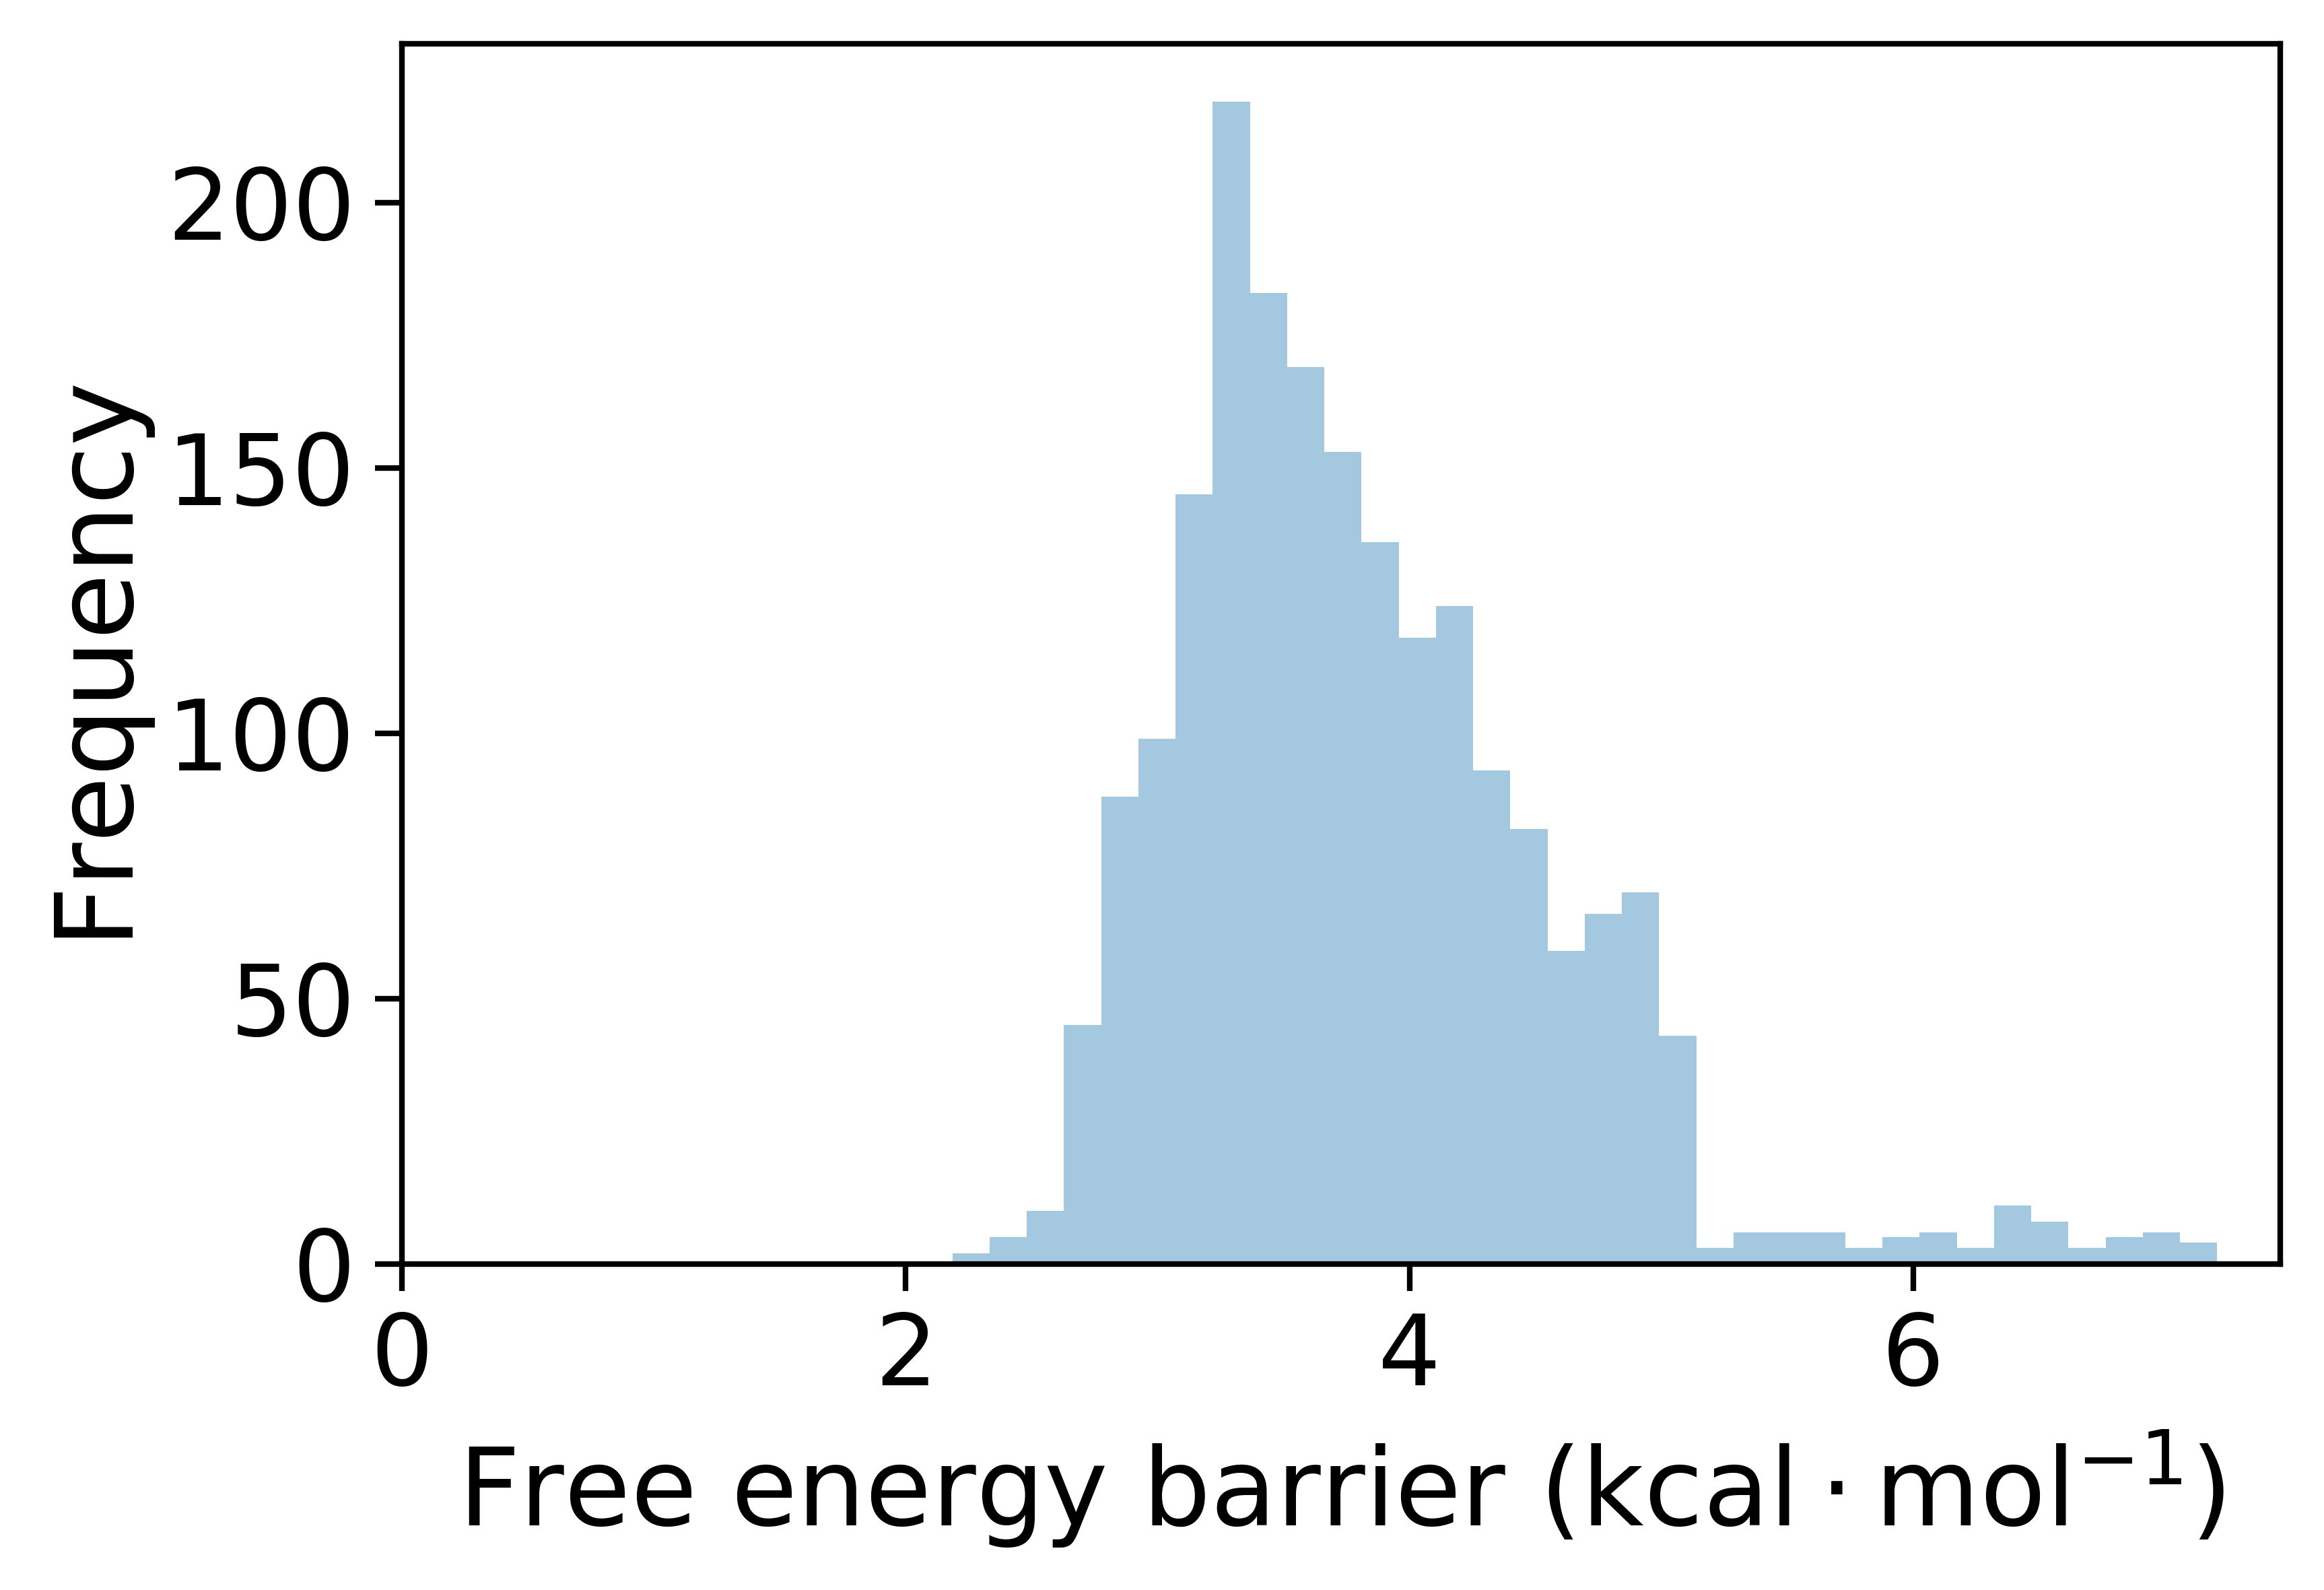
\includegraphics[width=0.8\textwidth]{chapters/water_hopping/figures/Fig_S10.png}
    \caption[Histogram of barrier heights for eight trajectories]{\textsc{Histogram of barrier heights for eight trajectories}. Barrier heights were calculated in \SI{1}{\nano\second} intervals. Free energies are calculated by converting the hopping timescales $(t)$ of the hidden Markov models to free energies $(\Delta G)$ using the transition-state theory expression for the hopping rate $k=1/t$: $\Delta G^{\mathrm{TS}}=R T \ln \left(k_{b} T \cdot t / h\right)$.}
    \label{fig:wat_s9}
\end{figure}

For each of the \num{947} \SI{1}{\nano\second} slices in local equilibrium, a HM model was constructed to determine the number of metastable states (cavities), the relative population of water within each cavity, transition probabilities for hopping between cavities, and the timescales for inter-cavity transport. The HM analysis shows that the cavities have a distribution of free energies (figure \ref{fig:wat_s9}), and a corresponding distribution of lifetimes for water within any given cavity. Figure \ref{fig:wat_f4}, panels (a) and (b) show representative examples from three \SI{1}{\nano\second} slices throughout one MD simulation where water hops between clusters of two and three cavities, along with information regarding the hopping timescales in subplots (ii). Subplots (iii) show the timescales of interstate rearrangement processes. These timescales do not correspond to pairwise hopping between cavities but rather joint relaxation processes over all states.


Extended periods of cavity hopping behaviour are found in all our \SI{300}{\kelvin} MD simulations: water repeatedly moves back and forth between adjacent cavities that do not fully collapse once they are vacated. The characteristic barriers for hopping between cavities have been calculated using transition state theory and are found to be on average $\num{6.42}\pm\num{1.29}k_{b}T$ ($\num{3.83}\pm\SI{0.77}{\kilo\cal\per\mol})$. The distribution across all trajectories (figure \ref{fig:wat_s9}) corresponds to a hop frequency of between \num{1} and \num{50} per nanosecond per water molecule, although not all hops will lead to productive diffusion against a concentration gradient. In fact, `return trips’ may be a common feature of water transport in these matrices.
Our analysis suggests that the magnitude of the S–E deviation depends on the transient packing efficiency of the organic molecules. For instance, raffinose self-diffuses slower than sucrose (hence the observed particle viscosity is higher), but if the average volume of cavity space within the lattice is larger and more highly connected, then the net water flux will be higher at a given particle viscosity. To evaluate this,  a series of MD simulations were carried out, which were post-analyzed to assess the cavity volume within glucose, sucrose and raffinose matrices. The final coordinates of the three matrices are presented in figure \ref{fig:wat_packing_eff}, showing increasing cavity size and density within the van der Waals surfaces. This quantity is also expressed as a fraction of the simulation volume in figure \ref{fig:wat_packing_eff}.

\begin{figure}
    \centering
    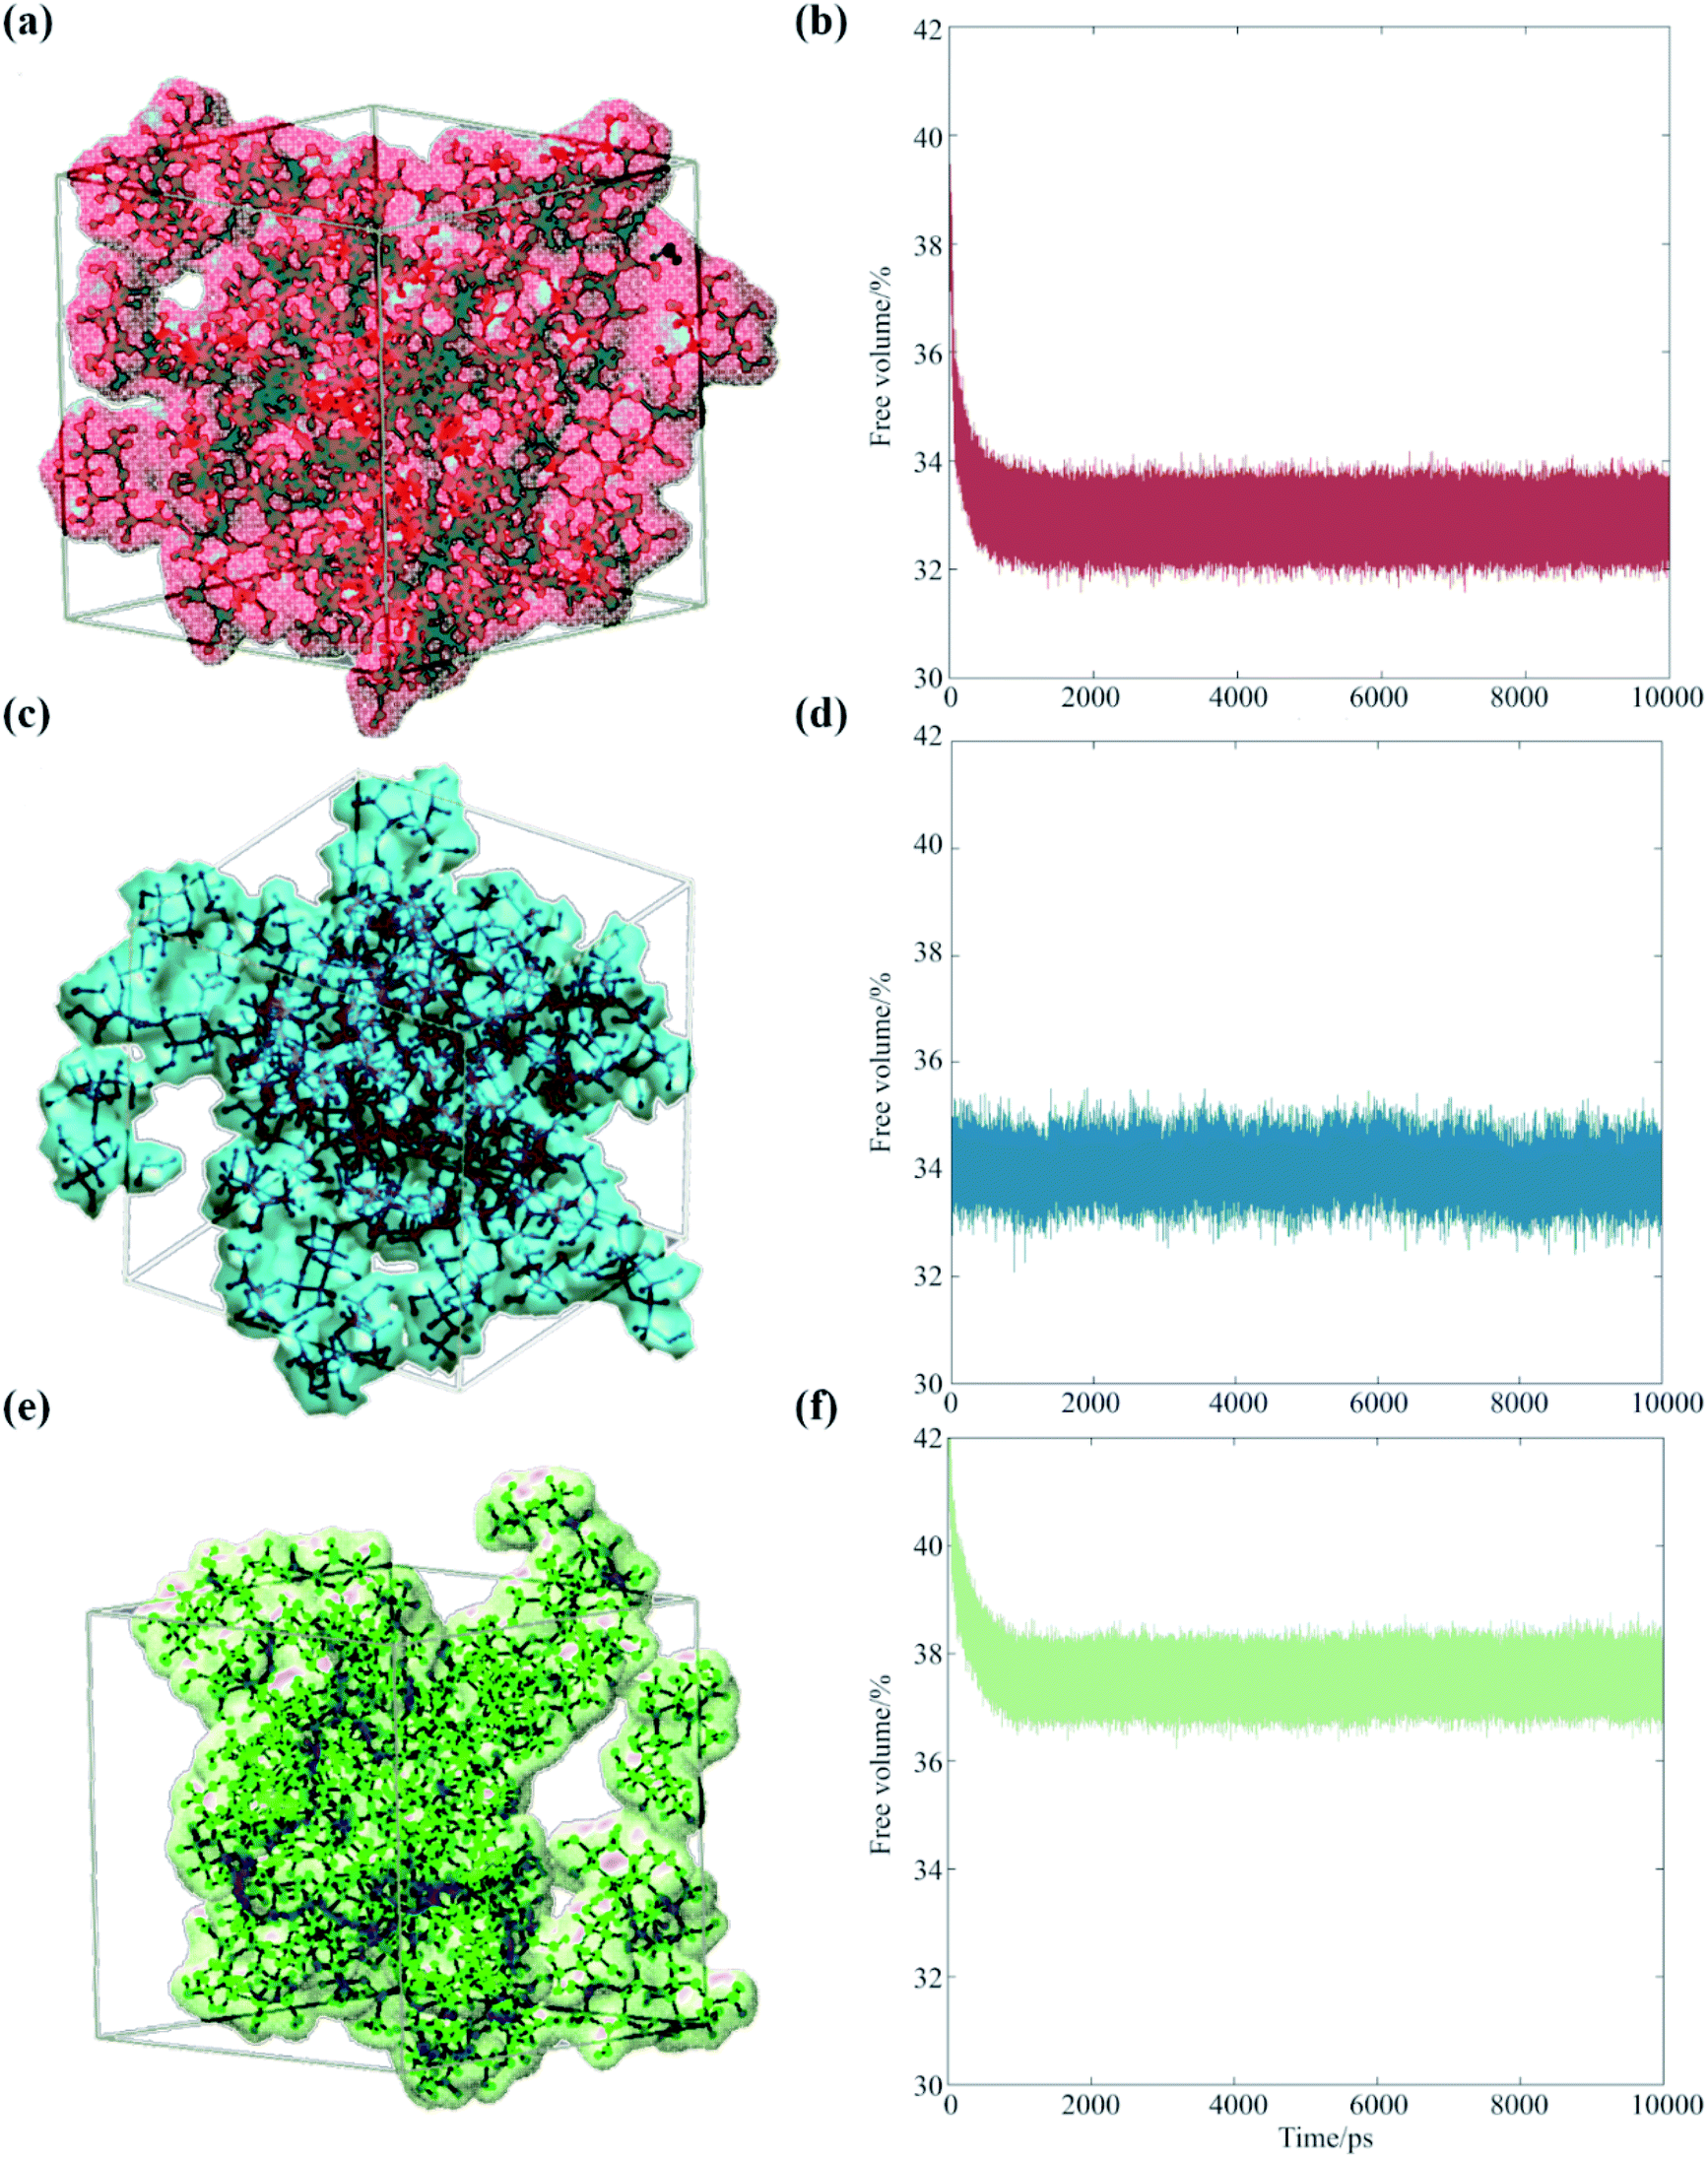
\includegraphics[width=0.8\textwidth]{chapters/water_hopping/figures/f5.png}
    \caption[Packing efficiency of organic molecules]{\textsc{Packing efficiency of organic molecules}. Occupied volumes of (a) glucose (\SI{67.1}{\percent}), (c) sucrose (\SI{66.0}{\percent}) and (e) raffinose (\SI{62.4}{\percent}) matrices are shown (same colour scheme as figure \ref{fig:wat_f1} again) showing the van der Waals radii of the saccharides within one snapshot of the short simulations. Fractional free volume are shown for (b) glucose, (d) sucrose, and (f) raffinose calculated by GROMACS throughout \SI{10}{\nano\second} simulations.}
    \label{fig:wat_packing_eff}
\end{figure}

Thus, the trend in viscosity data (figure \ref{fig:wat_f2}) can be rationalised at a molecular level: the `hopping’ mechanism of water transport will become more efficient as the size of the organic constituent increases. Therefore, the frictional forces experienced by water molecules will deviate further from those assumed by equation \ref{eqn:diffusion}, and the observed $D$ will be under-predicted to a greater extent for larger organics. With reference to atmospheric organic aerosol, this effect may be significant in particles containing large numbers of oligomeric or `humic-like’ molecules. Such constituents are frequently found in aerosol formed under low RH \cite{Jia2018}, low temperature \cite{huang2018alpha} or high precursor concentration \cite{Kourtchev2016} conditions.

\section{Conclusions}\label{sec:wat_conclusions}
In conclusion, this work has shown that the diffusion constant of water in viscous aerosol particles departs increasingly from the S-E equation as the size of the saccharide molecule forming the matrix increases. Atomistic simulations suggest that larger molecules will pack less efficiently, facilitating a mechanism of activated hopping through the porous network: at high saccharide fraction, a water molecule executes discrete jumps between cavities at a rate governed by the collective motion of the saccharide matrix. These observations also are consistent with the slower diffusion of molecules larger than water, whose motion more closely resembles that described by Stokes flow \cite{Gonzalez2015}.

The Markov modelling approach adopted here facilitated both the i) decomposition of a large amount of simulation data into tractable time-slices with an approximately stationary potential induced by the sucrose matrix; and ii) the quantitative description of kinetic processes involved in each slice. The results of applying the equilibrium assumptions to classify the time-slices resulted in only \SI{11.8}{\percent} being positively identified as being in local equilibrium.

A number of assumptions and approximations were made in order to facilitate this analysis. The first assumption was that the water dynamics could be approximated by considering a water molecule traversing a free energy surface arising from an static sucrose environment. This was was justified on the separation of timescales between the sucrose and water molecules. The estimated reorganisation time of \SI{1}{\nano\second}, over which this assumption was assumed to hold, pertains to the average movement of the sucrose molecule. However, fluctuations in parts of the sucrose molecule on the same timescale of the water motion were not ruled out. If present, these motions break the assumption that the kinetic rates of the water molecule were independent of time. These interactions were also left out of the variables used to describe kinetic states of the water molecule which limits the accuracy of eigenvectors of the Markov state model, i.e., some ``essential'' degrees of freedom were missing from the kinetic description. 

The second assumption was that, even if more rapid fluctuations of the sucrose molecule could be ruled out, the assumption of a universal reorganisation timescale of \SI{1}{\nano\second} was likely inaccurate. This results from two factors. First, this timescale was an average and thus deviation from this value are expected.  Second, even if deviations from an average reorganisation timescale are minimal, this particular figure is likely inaccurate because the sucrose reorganisation time was measured on a single sucrose molecule from a single trajectory by inspection of the autocorrelation function.  As a result, the proportion of time-slices described as being in equilibrium underestimates the true proportion of local equilibria. This is because it does not rule out local equilibria on time-slices shorter than \SI{1}{\nano\second} which may have then been incorrectly classified as out of equilibrium. Similarly, local equilibria may have lasted longer than \SI{1}{\nano\second} which would have allowed combining observations to produce a more precise estimate of the hopping timescales. 

The third assumption concerns the equilibration of the simulations. Each trajectory was equilibrated for \SI{500}{\pico\second} and measurement of the diffusion constant of water in the subsequent microsecond of simulation produced a value in agreement with the experimental measurements.  However, by their nature substances near the glass transition state have long equilibration times \cite{Bones2012}. It is possible that the rate of cavity formation and their size and shape could have changed over the course of the trajectories as the simulations continued to equilibrate after the initial \SI{500}{\pico\second}. Previous assumptions notwithstanding, this would not affect the validity of the Markov analysis because the trajectories were partitioned into stationary time-slices. However it may affect the distribution of hopping barriers and the measurement of diffusion constant.  

In addition, the modelling approach misses certain dynamical processes.  First, it does not say anything about the non-equilibrium processes which form the majority of the water transport. Second, the analysis of the equilibrium time-slices focused only on the slowest timescale processes in each time-slice. Multiple gaps in the eigenvalue spectrum were not identified which could have revealed further, faster timescale processes.  A plan to address these limitations in future work is laid out in the conclusions, chapter \ref{chap:conclusions}.

Despite this, the simplified Markov modelling approach used here, provided an insightful explanation of the diffusion of water within the saccharide matrix, in-line with experimental measurements and other simulation analysis. The models produced were successfully validated and visualisation of models from individual time-slices appeared consistent with the simulation data.  The simplified approach used intuition, visualisation and heuristics from the literature to guide the modelling process. The ``essential degrees of freedom'' - the Cartesian coordinates of the water molecule - were suggested by inspection of the molecular dynamics trajectories. The number of microstates followed a simple heuristic related to the volume of data, while the number of metastable states was determined from the eigenvalue spectrum. 




% \subsubsection{Markov state modelling}
% The goal of the Markov state modelling was to identify regions of the MD simulations in local equilibrium,to identify cavities,and calculate their associated hopping and relaxation timescales. Eight MD simulations were partitioned into \SI{1}{\nano\second} time-slices and the position of the water center of mass was clustered into $100$ discrete states using the k-means clustering algorithm. The k-means clustering and all subsequent calculations were performed using the open source software, PyEMMA30

% The discrete trajectories were screened to see whether they were in local equilibrium with the following procedure:
% \begin{enumerate}
%     \item A Markov state model (MSM) with a lag time ( $\tau$ ) of 10ps was constructed for each time-slice. The lag time was chosen so as to reveal details of potential metastability $^{31} .$ To determine the value of $\tau,$ we carried out a sensitivity analysis, varying $\tau$ until we observed convergence in the eigenvalues. See figure S10 panel (b \& f).
%     \item This MSM was coarse grained into a $k$ -state Hidden Markov Model (HMM) if the largest gap in successive implied timescales of the MSM $\left(t_{k} / t_{k+1}\right)$ was greater than 1.5. 
%     \item If the HMM had:
%     \begin{enumerate}
%         \item an absorbing state (a 1 on the diagonal of the transition matrix);
%         \item an metastable state, $i,$ with stationary distribution $\left(\pi_{i}\right)$ probability approximately zero $\left(\pi_{i}< 10^{-8}\right)$
%         \item negative eigenvalues; 
%     \end{enumerate}
%     it was classified as not being in local equilibrium.The conditions (a – c) are indicative of not being in equilibrium because of the enforcement of the detailed balance conditions when estimating the HMM transition matrix32
%     \item The time-slices identified as being in local equilibrium were used to construct a Bayesian HMM in order to estimate errors of the hopping timescales. 
% \end{enumerate}

% Out of the $8000$ time-slices analysed $947$ (\SI{11.8}{\percent}) were positively identified as being in local equilibrium. Figure S10 demonstrate this classification algorithm for two time-slices of trajectory 3. The first time-slice (\SIrange{0}{1}{\nano\second}, panels (a) to (d)) was classified as not being in local equilibrium, the second time-slice (\SIrange{22}{23}{\nano\second}, panels (e) - (h)) was classified as being in local equilibrium.

% \begin{figure}
%     \centering
%     \caption{\textbf{Position-position autocorrelation function of a single sucrose molecule within the simulation}. The plot shows very little motion in the region \SIrange{0.1}{1000}{\pico\second}.This plot suggests that it is reasonable cluster the data (to determine cavities, as in figure \ref{fig:wat_f4}) in increments of \SI{1}{\nano\second}. It is also reasonable to initialise frozen sucrose simulations after intervals of \SI{1}{\nano\second} (figure \ref{fig:wat_f3}, panels (b) - (d))}
%     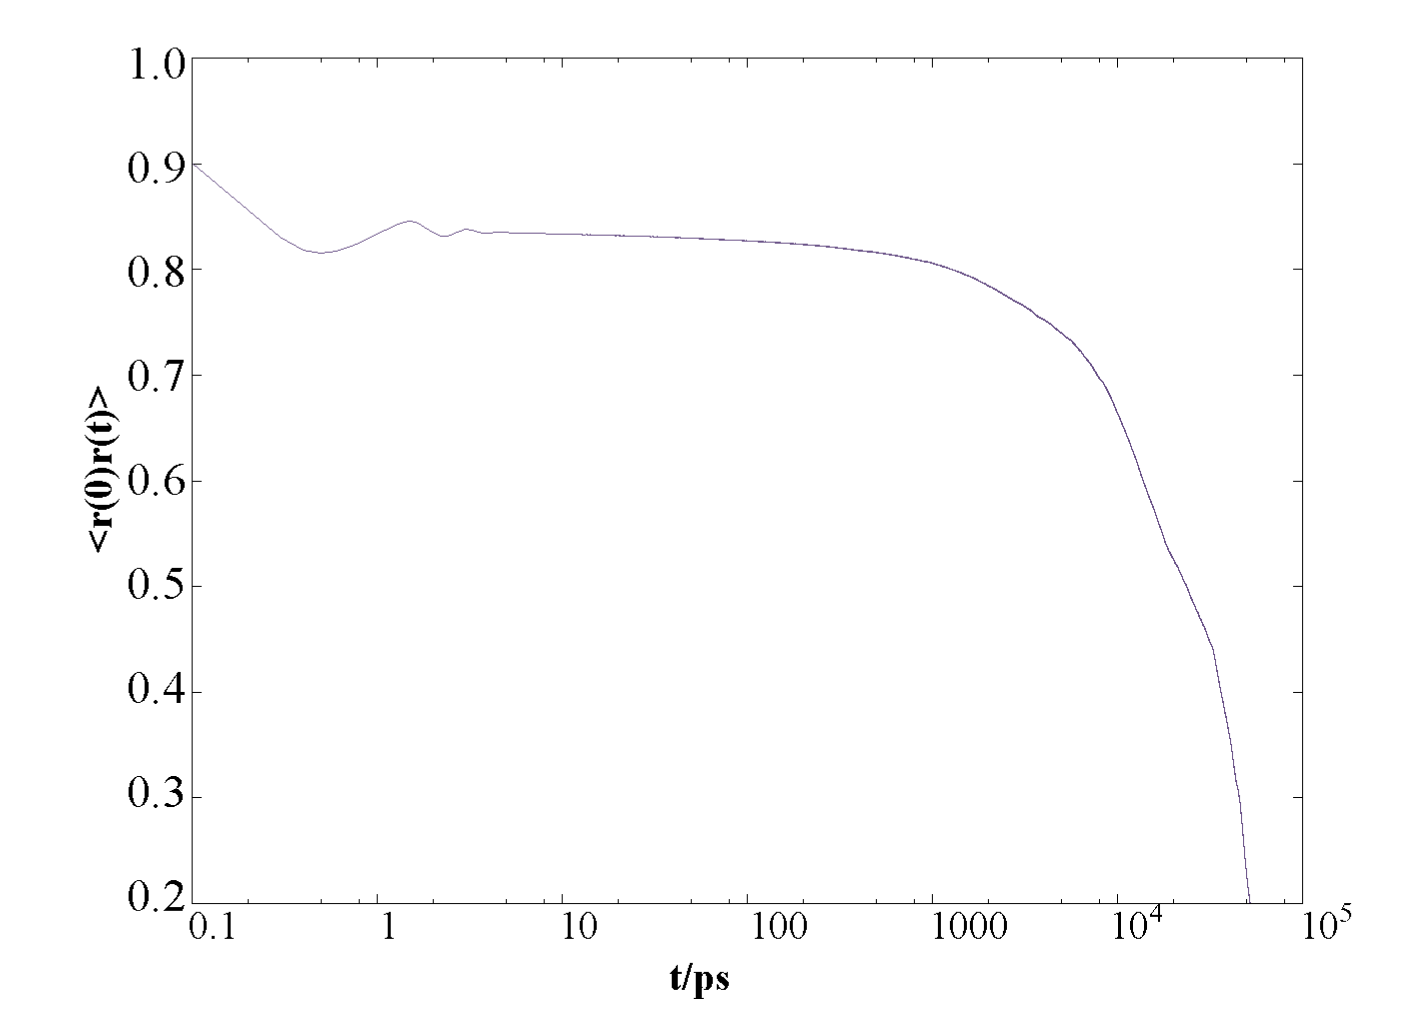
\includegraphics[width=0.8\textwidth]{chapters/water_hopping/figures/Fig_S8.png}
%     \label{fig:wat_s8}
% \end{figure}



% \begin{figure}[p]
%     \centering
%     \caption{\textbf{Classification of two time-slices from trajectory 3}: \SIrange{0}{1}{\nano\second} (panels (a) - (d), non-equilibrium time-slice) and \SIrange{22}{23}{\nano\second} (panels (e) - (h), local equilibrium time-slice). Panel (a) and (e) show the $x$, $y$, and $z$ coordinates of the center of mass of the water molecule. Panel (b) and (f) show the sensitivity analysis to determine the lag time $\tau$: the implied timescales, ($t$ vertical axis) vs the MSM lag, ($\tau$ horizontal axis). The black vertical line is place at \SI{10}{\pico\second} is the minimum time at which the implied timescales show convergence. Panels (c) and (g) show the stationary distribution. In panel (c) state $1$ has negligible probability classifying this time-slice as not being in equilibrium. Panels (d) and (h) show the attempted assignment of the discrete trajectory into metastable states. The non-equilibrium time-slice in panel (d) shows the large portion of unclassified states.}
%     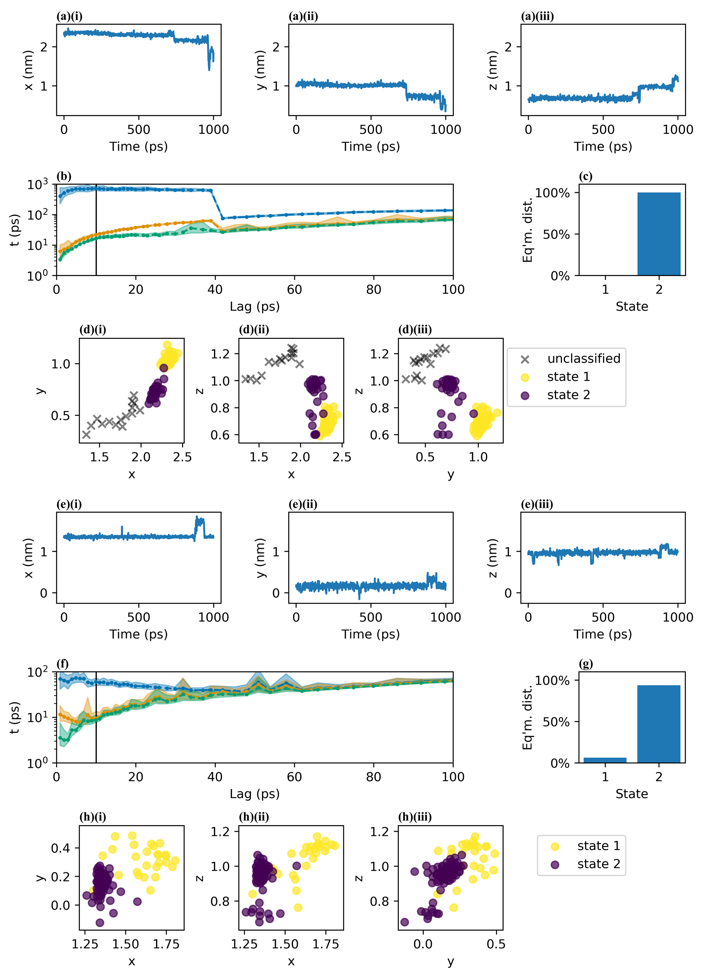
\includegraphics[width=0.8\textwidth]{chapters/water_hopping/figures/Fig_S11.png}
%     \label{fig:wat_s10}
% \end{figure}

% \section{Commentary and conclusions}\label{sec:wat_commentary}
% This work uses MMs in two different ways to understand the mechanism of water diffusion: first, by enforcing the equilibrium assumptions of stationarity and reversibility (from inspection of a HMM transition matrix and its eigenvalues/eigenvectors) to partition and classify the MD simulations into computationally tractable sub-trajectories. Second, by estimating a HMM on each sub-trajectory and calculating the slow relaxation timescales of the system. 

% The results of applying the equilibrium assumptions resulted in sub-trajectories of \SI{1}{\nano\second} with only \SI{11.8}{\percent} of these positively identified as being in local equilibrium. While this was done for computational simplicity, this means the majority of the simulation data is not used  and several improvements could be made. First, instead of using the average autocorrelation function to determine the sucrose rearrangement timescale, an adaptive strategy could be used to partition trajectories. Each time-slice is determined by the 



